\documentclass{article}
\title{Quarterly Report}

\linespread{1.2}
\usepackage[margin = 1.25 in]{geometry}
\usepackage{wrapfig}
\usepackage{amsfonts}
\usepackage[utf8]{inputenc}
\usepackage[T1]{fontenc}
\usepackage{graphicx}
\usepackage[english]{babel}
\usepackage[algoruled]{algorithm2e}

\renewcommand{\theequation}{\thesection.arabic{equation}}

\renewcommand{\thefigure}{\thesection.\arabic{figure}}



\renewcommand{\vec}[1]{\mathbf{#1}}
\renewcommand{\theequation}{\thesubsection.\arabic{equation}}
\DeclareGraphicsExtensions{.pdf,.png,.jpg, .gif}

\usepackage{amsthm}

\usepackage[english]{babel}
\usepackage{mathtools}

%\usepackage[OT2,T1]{fontenc}
%\DeclareSymbolFont{cyrletters}{OT2}{wncyr}{m}{n}
%\DeclareMathSymbol{\sha}{\mathalpha}{cyrletters}{"58}

\DeclareFontFamily{U}{wncy}{}
\DeclareFontShape{U}{wncy}{m}{n}{<->wncyr10}{}
\DeclareSymbolFont{mcy}{U}{wncy}{m}{n}
\DeclareMathSymbol{\Sh}{\mathord}{mcy}{"58} 
\DeclareMathOperator*{\argmin}{arg\,min}

\newcounter{eqn}
\renewcommand*{\theeqn}{\alph{eqn})}
\newcommand{\num}{\refstepcounter{eqn}\text{\theeqn}\;}

\makeatother
\newcommand{\vectornorm}[1]{\left|\left|#1\right|\right|}
\newcommand*\conjugate[1]{\bar{#1}}

\newtheorem{thm}{Theorem}
\newtheorem{defn}{Definition}
 %\theoremstyle{plain}
  \newtheorem{theorem}{Theorem}[section]
  \newtheorem{corollary}[theorem]{Corollary}
  \newtheorem{proposition}[theorem]{Proposition}
  \newtheorem{lemma}[theorem]{Lemma}
\newtheorem{example}[theorem]{Example}
  \newtheorem{definition}[theorem]{Definition}
  \newtheorem{conj}[theorem]{Conjecture}
 \newtheorem{condition}{Condition}
 \newtheorem{remark}[theorem]{Remark}

\newcommand{\supp}{\operatorname{supp}} 
\newcommand{\vc}[1]{{\mathbf{ #1}}}
\newcommand{\tn}{\widetilde{\nabla}_{n} }
\newcommand{\Z}{{\mathbb{Z}}}
\newcommand{\re}{{\mathbb{R}}}
\newcommand{\II}{{\mathbb{I}}}
\newcommand{\ep}{{\mathbb{E}}}
\newcommand{\pr}{{\mathbb{P}}}
\newcommand{\FF}{{\mathcal{F}}}
\newcommand{\TT}{{\mathcal{T}}}
\newcommand{\phin}{\phig{n}}
\newcommand{\phig}[1]{\phi^{(#1)}}
\newcommand{\ol}[1]{\overline{#1}}
\newcommand{\eff}{{\rm eff}}
\newcommand{\suc}{{\rm suc}}
\newcommand{\tends}{\rightarrow \infty}
\newcommand{\setS}{{\mathcal{S}}}
\newcommand{\setP}{{\mathcal{P}}}
\newcommand{\setX}{{\mathcal{X}}}
\newcommand{\nec}{{\rm nec}}
\newcommand{\bd}{{\rm bd}}

\begin{document}
\date{\today}
\author{Tom Kealy}
\maketitle
\section{Introduction}


\section{Models}

\subsection{Common Setup}
We are considering a radio environment with a single primary user (PU) and a network of \(J=\)50 nodes collaboratively trying to sense and reconstruct the PU signal, either in a fully distributed manner (by local message passing), or by transmitting measurements to a fusion centre which then solves the linear system. 

We are trying to sense and reconstruct a wideband signal, divided into \(L\) channels. We have a (connected) network of \(J\) (= 50) nodes placed uniformly at random within the square \(  \left[0,1\right]\times \left[0,1\right] \).

\subsection{Frequency Only}

\label{sensingmodel}
We are considering a radio environment with a single primary user (PU) and a network of \(J=\)50 nodes collaboratively trying to sense and reconstruct the PU signal, either in a fully distributed manner (by local message passing), or by transmitting measurements to a fusion centre which then solves the linear system. 

We are trying to sense and reconstruct a wideband signal, divided into \(L\) channels. We have a (connected) network of \(J\) (= 50) nodes placed uniformly at random within the square \(  \left[0,1\right]\times \left[0,1\right] \). They individually take measurements in the following way: by mixing the incoming analogue signal \(x\left(t\right)\) with a mixing function \(p_i\left(t\right)\) aliasing the spectrum. \(x\left(t\right)\) is assumed to be bandlimited and composed of up to \(k\) uncorrelated transmissions over the \(L\) possible narrowband channels - i.e. the signal is \(k\)-sparse. 

This process is repeated in parallel at each node (unrelated to \(N_{sig}\) so that each band in \(x\) appears in baseband. The mixing functions - which are independent for each node - are required to be periodic, with period \(T_p\). Since \(p_i\) is periodic it has Fourier expansion:

\begin{equation}
p_i\left(t\right) = \sum_{l=-\infty}^{\infty} c_{il} \exp\left({jlt\frac{2\pi}{T_p}}\right)
\end{equation}

The \(c_{il}\) are the Fourier coefficients of the expansion and are defined in the standard manner. The result of the mixing procedure in channel \(i\) is therefore \(xp_i\), with Fourier transform:

\begin{align}
X_{i}\left(f\right) &=& \int_{-\infty}^{\infty} x\left(t\right) p_i\left(t\right) dt
\\ &=& \sum_{l=-\infty}^{\infty} c_{il} X\left(f-lf_p\right)
\end{align}

(insert the Fourier series for \(p_i\), then exchange the sum and integral). The output of this mixing process then, is a linear combination of shifted copies of \(X\left(f\right)\), with at most \(\lceil f_NYQ/f_p\rceil\) terms since \(X\left(f\right)\) is zero outside it's support (we have assumed this Nyquist frequency exists, even though we never sample at that rate).

Once the mixing process has been completed the signal in each channel is low-pass filtered and sampled at a rate \(f_s \geq f_p\). In the frequency domain this is a ideal rectangle function, so the output of a single channel is:

\begin{equation}
Y_i\left(e^{j 2 \pi f T_s }\right) = \sum_{l = -L_0}^{+L_0}
\end{equation}

since frequencies outside of \([-f_2/2, f_s/2]\) will filtered out. \(L_0\) is the smallest integer number of non-zero contributions in \(X\left(f\right)\) over \([-f_2/2, f_s/2]\) - at most \(\lceil f_NYQ/f_p\rceil\) if we choose \(f_s = f_p\). These relations can be written in matrix form as:

\begin{equation}
\textbf{y} = \textbf{A}\textbf{x} + \vec{w}
\end{equation}

where \(\textbf{y}\) contains the output of the measurement process, and \(\textbf{A}\) is a product matrix of the mixing functions, their Fourier coefficients, a partial Fourier Matrix, and a matrix of channel co-efficients. \(\textbf{x}\) is the vector of unknown samples of \(x\left(t\right)\). 

i.e. \(\textbf{A}\) can be written: 

\begin{equation}
\textbf{A}^{m\times L} = \textbf{S}^{m\times L} \textbf{F}^{L\times L} \textbf{D}^{L \times L} \textbf{H}^{L \times L}
\label{system}
\end{equation}

The measurements \(\textbf{y}\) are transmitted to a Fusion Centre via a control channel. The system can then be solved by linear programming.

\subsection{Joint Space and Frequency}
We write the power spectral density (psd) of the \(sth\) transmitter as:

\begin{equation}
\phi_s = \sum_b \beta_{bs} \psi_b\left(f\right)
\label{basis_expansion}
\end{equation}
\\ 

This model expresses in psd of the transmitter in a suitable basis - for example \(\psi_b\left(f\right)\) could be zero everywhere except for the set of frequencies where \(f=b\) i.e. \(\psi\) is a rectangular function with height \(\beta_{bs}\) and support \(f\). Other candidates for \(\psi\) include splines (e.g. raised cosines), and complex exponentials. 

Given this, the psd at the \(rth\) receiver is:

\begin{equation}
\phi_r = \sum_s g_{sr}\phi_s = \sum_s g_{sr} \sum _b \beta_{bs}\psi_b\left(f\right)
\end{equation}

where

\begin{equation}
g_{sr} = \exp\left(-||x_r - x_s||_2^\alpha\right)
\end{equation}

is the channel response between the \(sth\) transmitter and the \(rth\) reciver.

This model can be summarised using Kronecker products as follows:

Let \(\tilde{G} = g_sr^T\), \(e_r, e_b\) be unit vectors i.e. they are \(1\) for the \(i^{th}\) receiver or frequency band respectively.

The received power at a receiver (when only a single transmitter is transmitting) can be written:

\begin{equation}
y_r = \left(	e_r^T \bigotimes I_{n_b}\right) y
\end{equation}

with,

\begin{equation}
y = \left( \tilde{G} \bigotimes I_{n_b} \right) \phi
\end{equation}

Now, we have

\begin{equation}
\phi = e_s \bigotimes \phi_s
\end{equation}

so,

\begin{equation}
y = \left( \tilde{G} \bigotimes I_{n_b} \right) \left(e_s \bigotimes \phi_s \right)
\end{equation}

finally we have,

\begin{equation}
y_r = \left(	e_r^T \bigotimes I_{n_b}\right)\left[\left( \tilde{G} \bigotimes I_{n_b} \right) \left(e_s \bigotimes \phi_s \right)\right]
\end{equation}

\(\beta_{bs} \in \re^{1 \times n_b}\), \(g_{sr} \in \re^{n_r \times n_s}\) and \(\psi_{kb} \in 1 \times n_k n_b\) where \(n_k\) is the number of frequency bands (in this example \(n_k = n_b\).

In the absence of knowledge of the location of the transmitters we introduce a grid of \textit{candidate} locations, to make the above model linear. \(s\) now runs over the set of these candidate locations.

The problem of estimating the coefficients, \(\beta\), from noisy observations \(y = \phi_r + N\left(0,1\right)\) is now one that can be tackled by linear regression/convex optimisation.


\section{Distributed Optimisation}
We now have a slight diversion into constrained convex optimisation, the denouement of which will not be apparent until later. This section follows (REF), and only contains enough to make the optimisation algorithm on graphs

Say, for example, that you are taking a walk up a mountain and would like to calculate the highest point along your path. You may then be tempted to solve a problem which looked like this:

\begin{equation*}
\begin{aligned}
& \underset{x}{\text{minimize}}
& & f\left( x \right) \\
& \text{subject to}
& & Ax = b
\label{orig_problem}
\end{aligned}
\end{equation*}

where \(f\) is a function in \(\re\), \(A \in \re^{n \times m}\) is a matrix, and \(x\in X\), \(X\) is some convex set.

This is a problem of constrained optimisation, which can be solved by adding a Lagrange multiplier like term to the unconstrained objective (which coincides with the constrained optimisation problem): 

\begin{equation}
L\left(x,y\right) = f\left( x \right) + y^T\left(Ax-b\right)
\end{equation}

where \(y\) is the Lagrange multiplier, and \(L\) is referred to as the Lagrangian. The components of \(y\) can be interpreted as the rate of change of the objective function as a function of the constraint variable. For example, if we are required to find the maximum height along a path on the mountain, the Lagrange multiplier would represent the rate of change in height along that specific path. 

We can find the solution of the original problem via the duality theorem of Fenchel:

\begin{equation}
g\left(y\right) = \inf_x L\left(x,y\right) = -f^*\left(-A^Ty\right) -b^Ty
\label{dual_problem}
\end{equation}

where \(f^*\) is the convex conjugate (Legendre-Fenchel) transform of \(f\). The problem is now to maximise \(g\). 

This maxima can be expressed in closed form as:

\begin{equation}
x^* = \underset{x}{\text{minimize}} L\left(x, y^*\right) 
\label{convex_soln}
\end{equation}

where \(y^*\) is the soln of the dual problem. 

Together \ref{dual_problem} and \ref{convex_soln} suggest a iterative algorithm, which proceeds iteratively by finding a minima of the objective function (up to a convex transformation) and then updating the Lagrange multiplier until some convergence criterion is met: 

\begin{align}
x^{k+1} &:= \underset{x}{\text{minimize}} L\left(x, y^*\right)  \\
y^{k+1} &:= y^{k} + \alpha^k \left(Ax^{k+1} - b\right)
\label{gradient_ascent}
\end{align}

This is a form of gradient ascent, with \( \alpha \) as the step size and \(k\) is the iteration counter. Assuming that \(g\) is differentiable, the algorithm is monotone (i.e. \( g\left(y^{k+1}\right) > g\left(y^{k}\right)\).

This algorithm is easily extended to the case where the objective function is linearly separable. That is scenarios where we can split \(f\left(x\right)\) into a sum of functions \(f_i\left(x_i\right)\), each over a disjoint domain \(x_i \in X_i\) (in our hill walking example, we can split our chosen path into a series of continuous intervals which lay next to each other). Extending the algorithm is simple: all that needs to be done is to perform the minimisation step in (\ref{gradient_ascent}) in each of the functions \(f_i\), and then jointly update the multiplier.

We have assumed the diferentiabilty \(g\) throughout, and it is this smoothness condition which allows the previous algorithm to terminate on a solution of the original constrained problem.

For problems with \(g\) not differentiable, the augmented Lagrangian is introduced as:

\begin{equation}
L_\rho\left(x,y\right) = f\left( x \right) + y^T\left(Ax-b\right) + \frac{\rho}{2}\|Ax-b\|_2^2
\end{equation}

where \(\rho\) is a penalty parameter. That is we're no longer seeking exact solutions, but instead seek solutions close in mean square error. 

The associated dual function is \(g_\rho\left(y\right) = \inf_x L_\rho\). By adding the penalty term, \(g_\rho\) is no differentiable, and the \(\rho \rightarrow 0\) regime corresponds to the solution of the original problem. 

The algorithm in this case can be found by first minimising over \(x\) and then evaluating the resulting equality constraint residual, i.e.:

\begin{align}
x^{k+1} &:= \argmin{x} L_\rho \\
y^{k+1} &:= y^{k} + \rho \left(Ax^{k+1} - b\right)
\label{mom}
\end{align}

This algorithm is known as the method of multipliers for solving the problem (\ref{orig_problem}). Note that even if \(f\) is separable, the augmented Lagrangian may not be.

\subsubsection{ADMM}
The alternating direction method of multipliers (ADMM), is an algorithm intended to blend the decomposability of the gradient ascent algorithm \ref{gradient_ascent}, with the more general method of multipliers \ref{mom}, i.e. when the objective function is decomposable but the dual function is not differentiable. The algorithm solves problems of the form

\begin{align}
\text{min}_{x} f\left( x \right) + g\left(z\right)
\\
\text{s.t } Ax +Bz = c
\label{admm}
\end{align}

where \(f\) and \(g\) are assumed to be convex function with range in \(\re\), \(A \in \re^{p \times n}\) and \(B\in \re^{p \times m}\) are matrices (not assumed to have full rank), and \(c \in \re^p\). We begin by illustrating a few examples, relevant to the type of problems encountered in signal processing.

\begin{example}
The Basis Pursuit problem

\begin{equation*}
\begin{aligned}
& \underset{x}{\text{minimize}}
& & \|x\|_1 \\
& \text{subject to}
& & Ax = b
\label{bp}
\end{aligned}
\end{equation*}

can be written in the ADMM form (\ref{admm}):

\begin{equation*}
\begin{aligned}
& \underset{x}{\text{minimize}}
& & f\left( x \right) + \|z\|_1 \\
& \text{subject to}
& & x - z = 0
\label{bp_reform}
\end{aligned}
\end{equation*}

where \(f\) is the indicator function of \(\{x\in \re^n : Ax = b\}\). 

\end{example} 

\begin{example}
Similarly the LASSO:

\begin{equation}
\text{minimise } \frac{1}{2}\|Ax-b\|_2^2 + \lambda\|x\|_1
\end{equation}

\(\lambda > 0\), can be solved by the ADMM with \(f = \frac{1}{2}\|Ax-b\|_2^2\) and \(g = \lambda\|x\|_1\).

\end{example}

The solution of (\ref{admm}) is:

\begin{equation}
x* = \inf\{f\left( x \right) + g\left(z\right) : Ax +Bz = c\}
\end{equation}

As previously we form the Lagrangian:

\begin{equation}
L_\rho\left(x,y\right) = f\left( x \right) + g\left(z\right) + y^T\left(Ax+Bz-c\right) + \frac{\rho}{2}\|Ax+Bz-c\|_2^2
\end{equation}

ADMM consists of the iterations:

\begin{align}
x^{k+1} &:= \argmin{x} L_\rho\left(x,z^k,y^k\right)\\
z^{k+1} &:= \argmin{z} L_\rho\left(x^{k+1},z,y^k\right)\\
y^{k+1} &:= y^{k} + \rho \left(Ax^{k+1} + Bz^{k+1} - c\right)
\label{admm_algo}
\end{align}

Note that this algorithm is similar to both the gradient ascent and method of multipliers from the last section: it has an \(x\) minimisation step, an \(z\) minimisation step and a dual variable update. I.e. the Lagrangian is updated simultaneously with respect to the two primal variables. Separating minimisation into two steps (as opposed to joint minimisation) is what allows for decomposition if \(f\) or \(g\) (or both) are separable. 

\subsection{Example: Consensus}
Suppose we want to solve a problem such as:

\begin{equation*}
\begin{aligned}
& \underset{x}{\text{minimize}}
& & \sum_i f_i\left( x \right) \\
\label{consensus}
\end{aligned}
\end{equation*}

this could arise in statistical computing where \(f_i\) would be the loss function for the \(i^th\) block of training data. We can write the problem for distributed optimisation as:

\begin{equation*}
\begin{aligned}
& \underset{x}{\text{minimize}}
& & \sum_i f_i\left( x_i \right) \\
& \text{subject to}
& & x_i - z = 0
\label{admm_consensus}
\end{aligned}
\end{equation*}

where \(x_i\) are local variables (for example local to each node in a spectrum sensing) and \(x_i - z = 0\) are the consensus constraints. Consensus and regularisation can be achieved by adding a regularisation term \(g\left(z\right)\) - for example \(g\left(z\right) = \lambda||x||_1\) corresponds to the LASSO, and the \(f_i\) would be \(f_i = ||A_ix_i - b||_2^2\). 

As per the previous sections, we form the Augmented Lagrangian:

\begin{equation}
L_\rho\left(x,y\right) = \sum_i^n \left(f_i\left( x_i \right) + y_i^T\left(x_i-z\right) + \frac{\rho}{2}\|x_i-z\|_2^2\right)
\end{equation}

The ADMM iterations for this Lagrangian are:

\begin{align}
x_i^{k+1} &:= \argmin{x_i} \left(f_i\left( x_i \right) + y_i^{kT}\left(x_i-z\right) + \frac{\rho}{2}\|x_i-z\|_2^2\right)\\
z^{k+1} &:= \frac{1}{n}\sum_i^n \left(x_i^{k+1} + \left(1\rho\right)y_i^k\right)\\
y_i^{k+1} &:= y_i^{k} + \rho \left(x_i^{k+1} - z^{k+1} \right)
\label{consensus_iterations}
\end{align}

The \(z^{k+1}\) iteration is analytic as we're minimising the squared norm of \(x_i - z\) - so we average. With \(\|x\|_1\) regularisation we perform soft-thresholding after the \(z\) update.

At each iteration the sum of the dual variables \(y_i\) is zero, so the algorithm can be simplified to:

\begin{align}
x_i^{k+1} &:= \argmin{x_i} \left(f_i\left( x_i \right) + y_i^{kT}\left(x_i-\bar{x}^k\right) + \frac{\rho}{2}\|x_i-\bar{x}^k\|_2^2\right)\\
y_i^{k+1} &:= y_i^{k} + \rho \left(x_i^{k+1} - z^{k+1} \right)
\label{simple_consensus_iterations}
\end{align}
 
where

\begin{equation}
\bar{x}^k = \frac{1}{n} \sum_i^n x_i^k
\end{equation}

This algorithm can be summarised as follows: in each iteration

\begin{itemize}
\item gather \(x^k\) and average to get \(\bar{x}^k\)
\item scatter the average to nodes
\item update \(y_i^k\) locally
\item update \(x_i\) locally
\end{itemize}

Each agent is minimising it's own function, plus a quadratic term (the squared norm) which penalises the agent from moving too far from the previous average.

Note that the 'gather' stage doesn't require a central processor - this can be done in a distributed manner also.

\subsection{statistical interpretation}
At each step \(k\) of the algorithm each agent is minimising it's own loss function, plus a quadratic.
This has a simple interpretation: we're doing MAP estimation under the prior \(\mathcal{N}\left(\bar{x}^{k} + \left(1\rho\right)y_i^k, \rho I\right)\). I.e. the prior mean is the previous iteration's consensus shifted by node \(i\) disagreeing with the previous consensus. 

I think what's going on is that after some (large) number of steps \(k*\) we can replace the prior iteration mean with the 'optimal' mean i.e. \(|x_i^{k*} - \bar{x*}| \leq \varepsilon \), and taking a convex combination of these \(x_j^{k*} \forall j \in \{1\ldots n\}\) we get a slightly better estimate because for any finite \(k\) large enough not all the \(x_j\) will be the same.

I think that when we add regularisation, we change the prior to a Laplace prior, with parameters corresponding to the previous iteration. 

\subsection{Constrained Optimisation on Graphs}
We model the network as an undirected graph \(G = \left(V,E\right)\), where \(V = \{1 \ldots J\}\) is the set of vertices, and \(E = V \times V\) is the set of edges. An edge between nodes \(i\) and \(j\) implies that the two nodes can communicate. The number of nodes node \(i\) can communicate is written \(\mathcal{N}_i\) and the degree of node \(i\) is \(D_i = |\mathcal{N}_i|\). 

We assume that a proper (or approximate) colouring of the graph is available: that is each node is assigned a number from a set \(C = \{1 \ldots c \} \), and no node shares a colour with any neighbour.

Given the measurement model from the section (SECTION), we can represent the linear system by concatenating the measurements of each node into a single system. Where, each row of the matrix represents the measurements of a single node. I.e we are trying to solve the following problem:

\begin{equation}
\text{min} ||x||_1 \text{ subject to } A_p x = b_p
\end{equation}

The problem is coupled at each node by the variable \(x\). To ease this issue, at each node create a local copy, denoted \(x_j\) (so there will be \(J\) copies of this variable). 

Then, for consistency, we constrain the problem, so that each copy is identical: \(x_1 = x_2 = \ldots x_J\). Equivalently, given the graphical structure of the problem, we require that \(x_i = x_j\) for each edge of the network.

So now we are solving the problem

\begin{equation}
\text{min} \frac{1}{J}\sum_J||x_j||_1 \text{ subject to } A_p x = b_p \text{ and } x_i = x_j \{i,j\} \in E 
 \label{constrainedbp}
\end{equation}
 
This is exactly the kind of problem that can be attacked by the Alternating Direction Method of Multipliers, described previously. We present a short example for bipartite graphs, which can easily be generalised to graphs with many colours. 
 
\subsection{Example: bipartite graphs}
We are here considering graphs which are connected, and 2-colourable, that is nodes 1 to \(c\) have colour 1 (red say), and nodes \(c+1\) to \(J\) have colour 2 (blue). We will demonstrate that we can decompose problem (\ref{constrainedbp}) into \(c\) problems which can be executed in parallel by minimising \(x\) at the 1st set of nodes, and \(J - c\) problems which also can be executed in parallel by minimising at the second set of nodes. 

Firstly, for compactness, we introduced the arc-incidence matrix of the graph \(B\). This is the \(J \times E\) matrix where each column corresponds to an edge \(\{i,j\} \in E\), with the \(ith\) and \(jth\) entries equal to 1 and -1 respectively. With this notation, we can rewrite (\ref{constrainedbp}) as:

\begin{equation}
\text{min} \frac{1}{J}\sum_J||x_j||_1 \text{ subject to } A_p x = b_p \text{ and } \left(B^T \circ I \right)\bar{x} = 0 
 \label{constrainedbp1}
\end{equation}

where \(\bar{x} = \left(x_1, x_2, \ldots x_J \right)\), and \(\circ\) is the Kronecker product. 

In this form, the Lagrangian of the problem (\ref{constrainedbp1}) can be written in the following way:

\begin{align}
L\left(\bar{x}_1, \bar{x}_2; \lambda\right) = \frac{1}{J}\sum_{j \in C_1}||x_j||_1 + \frac{1}{J}\sum_{j \in C_2}||x_j||_1 &+ \\ \phi_1\left(\bar{x_1}, \lambda\right) + \phi_2\left(\bar{x_2}, \lambda\right) &+ \\
\rho\bar{x}_1^T\left(B_1B_2^T\circ I_n\right)\bar{x}_2
\end{align}
where 

\begin{align}
\phi_i\left(\bar{x}_i, \lambda\right) &= \lambda^T\left(B_i^T\circ I_n\right)\bar{x}_i + \frac{\rho}{2}\vectornorm{\left(B_i^T\circ I_n\right)\bar{x}_i }^2 \\
&= \left(\left(B_i^T\circ I_n\right)\lambda \right)^T\bar{x}_i + \frac{\rho}{2}\bar{x}_i^T\left(B_1B_2^T\circ I_n\right)\bar{x}_i
\end{align}

Since, no nodes within \(C_i\) are neighbours \(B_iB_i^T\) is a diagonal matrix (with the degree of node \(i\) as the \(i\)th entry). So, we can finally re-write

\begin{equation}
\phi_i\left(\bar{x}_i, \lambda\right) = \sum_{j \in C_i}\left(\left(\sum_{k \in \mathcal{N}_i} sign\left(k-i\right)\lambda_{\{i,k\}}\right)^T x_i + \frac{\rho}{2}D_i\vectornorm{x_i}^2  \right)
\end{equation}

where the dual variable \(\lambda\) has been decomposed edge-wise so that \(\lambda_{\{i,j\}} = \lambda_{\{j,i\}}\) and is associated with edge \(\{i,j\}\) and the constraint \(x_i = x_j\).

\section{Results}

\subsection{Frequency only Model}

The model described in section (\ref{sensingmodel}) was simulated, 

\begin{figure}[h]
\centering
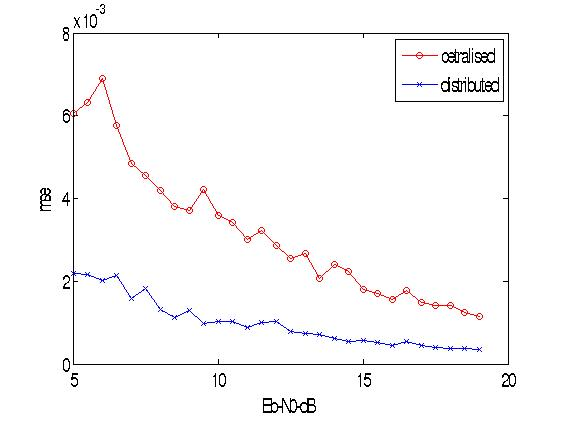
\includegraphics[height = 5 cm]{centvsdistmsegaussian10perpoint.jpg}
\caption{Mse vs SNR for the 'frequency only sensing model, showing the performance of distributed and centralised solvers}
\label{msevssnr1}
\end{figure}

\begin{figure}[h]
\centering
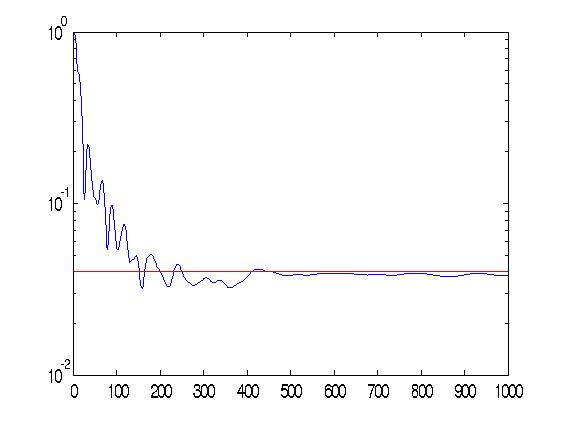
\includegraphics[height = 5 cm]{erroriterations1.jpg}
\caption{The progress of a distributed and a centralised solver as a function of the number of iterations }
\label{erroriterations}
\end{figure}

\subsection{Joint Space-Frequency}

\begin{figure}[h]
\centering
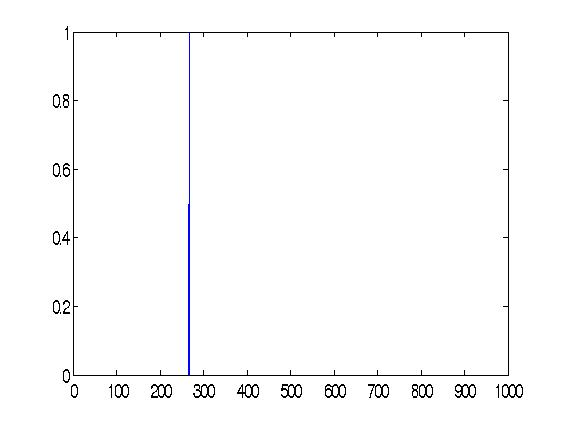
\includegraphics[height = 5 cm]{betabs.jpg}
\caption{Example of \(\beta_{bs}\) for the 'joint space-frequency' model}
\label{beta}
\end{figure}

\begin{figure}[h]
\centering
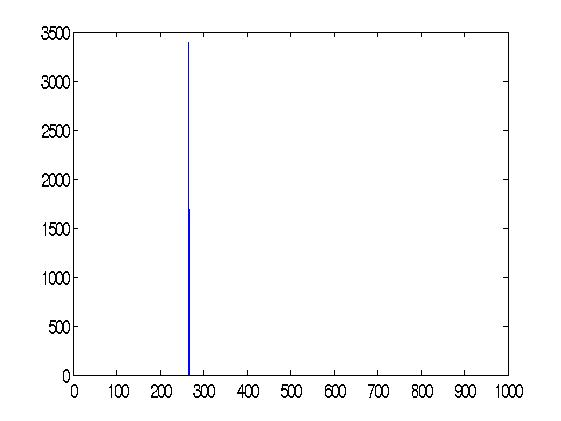
\includegraphics[height = 5 cm]{node1.jpg}
\caption{\(\beta_{bs}\) as seen by a node after a round o ADMM}
\label{betanode}
\end{figure}

\begin{figure}[h]
\centering
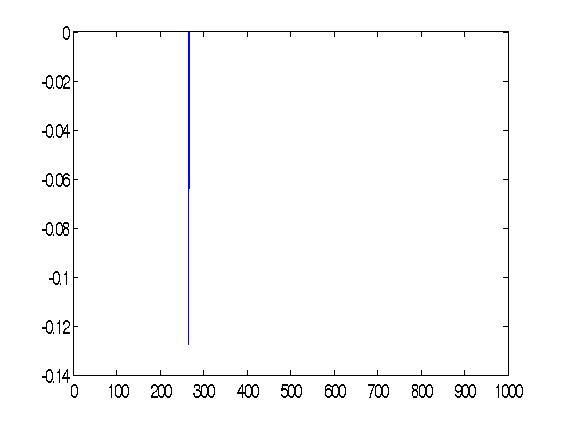
\includegraphics[height = 5 cm]{spatialcentral.jpg}
\caption{\(\beta_{bs}\) as produced by the centralised solver spgl1}
\label{betacentral}
\end{figure}

\begin{figure}[h]
\centering
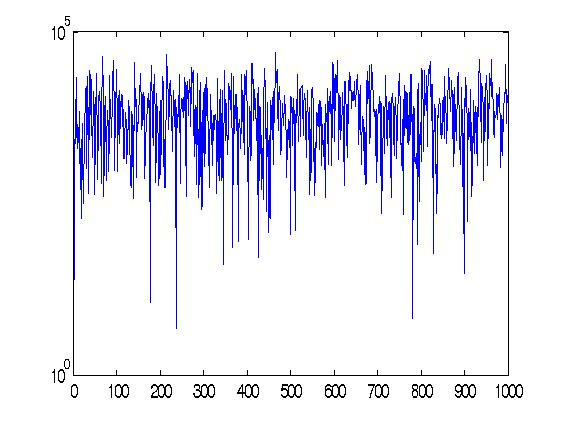
\includegraphics[height = 5 cm]{spatialiterations.jpg}
\caption{The progress of ADMM as a function of iterations for the joint model}
\label{spatialiterations}
\end{figure}

\section{Conclusions and Further Work}

\end{document}